\chapter{Regulator}
\label{cha:regulator}

W zaprojektowanym układzie kamera pełni rolę sensora uchybu regulacji.
Układ nie ma możliwości mierzenia pozycji serwomechanizmów. Planowane jest dodanie tej funkcjonalności w przyszłości (prawdopodobnie luty 2017).
%TODO Może napisać, że jest to planowane kiedyś tam. -zrobione.
Aby zagwarantować poprawne pozycjonowanie zbudowanej głowicy obrotowej należy więc zaimplementować regulator, którego wyjściem będzie wartość zadana serwomechanizmów.

\section{Model układu}
\label{sec:modelukladu}

Aby mieć możliwość testowania regulatora bez konieczności każdorazowej zmiany kodu źródłowego oraz ryzyka uszkodzenia układu postanowiono wyznaczyć model układu, a następnie przeprowadzić badania symulacyjne w programach \textit{MATLAB} i \textit{Simulink}.
Na podstawie modelu można również dobrać parametry regulatora, które zapewnią asymptotyczną stabilność oraz szybkie pozycjonowanie układu.
Prace rozpoczęto od wyznaczenia transmitancji serwomechanizmów. Wiadomo, że w urządzeniu zastosowano regulator proporcjonalny.
Schemat blokowy serwomechanizmu przedstawiony został na rysunku \ref{fig:servo}.

\begin{figure}[h]
	\centering
	\includegraphics[width=4in]{servo.jpg}
	\caption{Schemat blokowy serwomechanizmu.}
	\label{fig:servo}
\end{figure}
%TODO ref do rysnku w txt -zrobione.

\noindent Gdzie:\newline
\(G_o(s)\) jest transmitancją silnika prądu stałego, gdy wejściem jest napięcie, a wyjściem położenie kątowe wału silnika:
\begin{equation}
G_o(s)=\frac{1}{s(Ts+1)}
\end{equation}
%TODO czegoś w tym zadniu brakuje ?
\(K\) jest wzmocnieniem regulatora proporcjonalnego.\newline
Transmitancja zastępcza powyższego układu wynosi:
\begin{equation}
\label{eq:servo}
G_s(s)=\frac{K}{Ts^2+s+K}
\end{equation}
Ze względu na brak enkoderów w układzie, nie można przeprowadzić identyfikacji parametrów serwomechanizmów.
Na podstawie obserwacji wiadomo, że w wzmocnienie regulatora jest dobrane tak, by silnik nie oscylował wokół wartości zadanej.
Powinno być ono wzmocnieniem krytycznym dla danego silnika.
Aby wzmocnienie \(K\) było krytyczne, musi być ono równe:
\begin{equation}
\label{eq:kryt}
K=\frac{1}{4T}
\end{equation}
Podstawiając powyższy wzór do równania (\ref{eq:servo}) otrzymuje się:
\begin{equation}
G_s(s)=\frac{1}{4T^2s^2+4Ts+1}
\end{equation}
Wartość stałej czasowej jest przyjęta na podstawie odpowiedzi skokowej serwomechanizmu.
\begin{equation}
T=0.05
\end{equation}
Następnie wykonano schemat blokowy kompletnego układu (z kamerą i implementowanym regulatorem).
Przedstawiony on został na rysunku \ref{fig:uklad}.

\begin{figure}[h]
	\centering
	\includegraphics[width=4in]{uklad.jpg}
	\caption{Schemat blokowy kompletnego układu.}
	\label{fig:uklad}
\end{figure}
%TODO ref. -zrobione.

\(G_R(z)\) jest transmitancją projektowanego regulatora dyskretnego.
\paragraph*{}
Rolę przetwornika A/D pełni w układzie kamera, a przetwornika D/A sterownik serwomechanizmów. 
Schemat ten można przedstawić w równoważnej postaci, przedstawionej na rysunku \ref{fig:uklad_digital}.

\begin{figure}[h]
	\centering
	\includegraphics[width=4in]{uklad_digital.jpg}
	\caption{Równoważny schemat kompletnego układu.}
	\label{fig:uklad_digital}
\end{figure}
%TODO ref. -zrobione.

Transmitancję opisaną równaniem (\ref{eq:servo}) można zapisać za pomocą równań stanu:
\begin{equation}
\dot{x}=Ax+Bu
\end{equation}
\begin{equation}
y=Cx
\end{equation}
\begin{equation}
A=
	\begin{bmatrix}
	0 & 1 \\
	-\frac{K}{T} & -\frac{1}{T}
	\end{bmatrix}
\end{equation}
\begin{equation}
B=
	\begin{bmatrix}
	0 \\
	1
	\end{bmatrix}
\end{equation}
\begin{equation}
C=
	\begin{bmatrix}
	\frac{K}{T} & 0
	\end{bmatrix}
\end{equation}
Wzmocnienie krytyczne regulatora w serwomechanizmach dobrane jest dla silników bez obciążenia. 
Jeśli silnik zostaje obciążony, to zwiększa się jego stała czasowa. 
Wzmocnienie więc również powinno być zmienione. 
Wziąć należy jednak pod uwagę, że masa użytej kamery jest mała w porównaniu do maksymalnej masy obciążenia tych urządzeń. 
Z tego względu można przyjąć, że stała czasowa nie zmienia się, a wzmocnienie nadal jest krytyczne. 
Równanie (\ref{eq:kryt}) jest więc nadal spełnione. 
%TODO zachodzi równanie ? poza tym odwołania do równań w () -zrobione.
Podstawiono je do powyższych macierzy.
\begin{equation}
A=
	\begin{bmatrix}
	0 & 1 \\
	-\frac{1}{4T^2} & -\frac{1}{T}
	\end{bmatrix}
\end{equation}
\begin{equation}
B=
	\begin{bmatrix}
	0 \\
	1
	\end{bmatrix}
\end{equation}
\begin{equation}
C=
	\begin{bmatrix}
	\frac{1}{4T^2} & 0
	\end{bmatrix}
\end{equation}
Obiekt ten można razem z przetwornikiem A/D i przetwornikiem D/A pierwszego rzędu przedstawić można jako jeden równoważny obiekt dyskretny. Wyznaczono następnie równania stanu tego obiektu \cite{TS}.
\begin{equation}
\label{eq:A^+}
A^+=e^{hA}
\end{equation}
\begin{equation}
\label{eq:B^+}
B^+=\int\limits_{0}^{h}e^{tA}Bdt
\end{equation}
\begin{equation}
C^+=C
\end{equation}
\(h\) oznacza okres próbkowania dyskretnej części układu.
\begin{equation}
h=\frac{1}{60}
\end{equation}
Obliczenia rozpoczęto od wyliczenia macierzy \(e^{tA}\).
\begin{equation}
e^{tA}=\mathcal{L}^{-1}[(sI-A)^{-1}]
\end{equation}
\begin{equation}
e^{tA}=\mathcal{L}^{-1}
	\begin{bmatrix}
	\frac{s+\frac{1}{T}}{(s+\frac{1}{2T})^2} & \frac{1}{(s+\frac{1}{2T})^2} \\
	\frac{-\frac{1}{4T^2}}{(s+\frac{1}{2T})^2} &  \frac{s}{(s+\frac{1}{2T})^2}
	\end{bmatrix}
\end{equation}
\begin{equation}
\label{eq:e^tA}
e^{tA}=
	\begin{bmatrix}
	(1+\frac{t}{2T})e^{-\frac{t}{2T}} & te^{-\frac{t}{2T}} \\
	-\frac{t}{4T^2}e^{-\frac{t}{2T}} & (1-\frac{t}{2T})e^{-\frac{t}{2T}}
	\end{bmatrix}
\end{equation}
Podstawiono \ref{eq:e^tA} do \ref{eq:A^+} i \ref{eq:B^+}.
\begin{equation}
A^+=
	\begin{bmatrix}
	(1+\frac{h}{2T})e^{-\frac{h}{2T}} & he^{-\frac{h}{2T}} \\
	-\frac{h}{4T^2}e^{-\frac{h}{2T}} & (1-\frac{h}{2T})e^{-\frac{h}{2T}}
	\end{bmatrix}
\end{equation}
\begin{equation}
B^+=\int\limits_{0}^{h}
	\begin{bmatrix}
	te^{-\frac{t}{2T}} \\
	(1-\frac{t}{2T})e^{-\frac{t}{2T}}
	\end{bmatrix}
	dt
\end{equation}
\begin{equation}
\int te^{-\frac{t}{2T}}=-2Tte^{-\frac{t}{2T}}+2T\int e^{-\frac{t}{2T}}dt
\end{equation}
\begin{equation}
\int te^{-\frac{t}{2T}}=-2Tte^{-\frac{t}{2T}}-4T^2e^{-\frac{t}{2T}}
\end{equation}
\begin{equation}
B^+=
	\begin{bmatrix}
	-2T(h+2T)e^{-\frac{h}{2T}}+4T^2 \\
	he^{-\frac{h}{2T}}
	\end{bmatrix}
\end{equation}
\begin{equation}
C^+=
	\begin{bmatrix}
	\frac{1}{4T^2} & 0
	\end{bmatrix}
\end{equation}
Aby sprawdzić poprawność przeprowadzonych obliczeń postanowiono porównać odpowiedzi skokowe układu ciągłego i dyskretnego. Do tego celu zostało wykorzystane środowisko \textit{MATLAB}. Porównanie to zostało przedstawione na rysunku \ref{fig:comp}.

\begin{figure}[h]
	\centering
	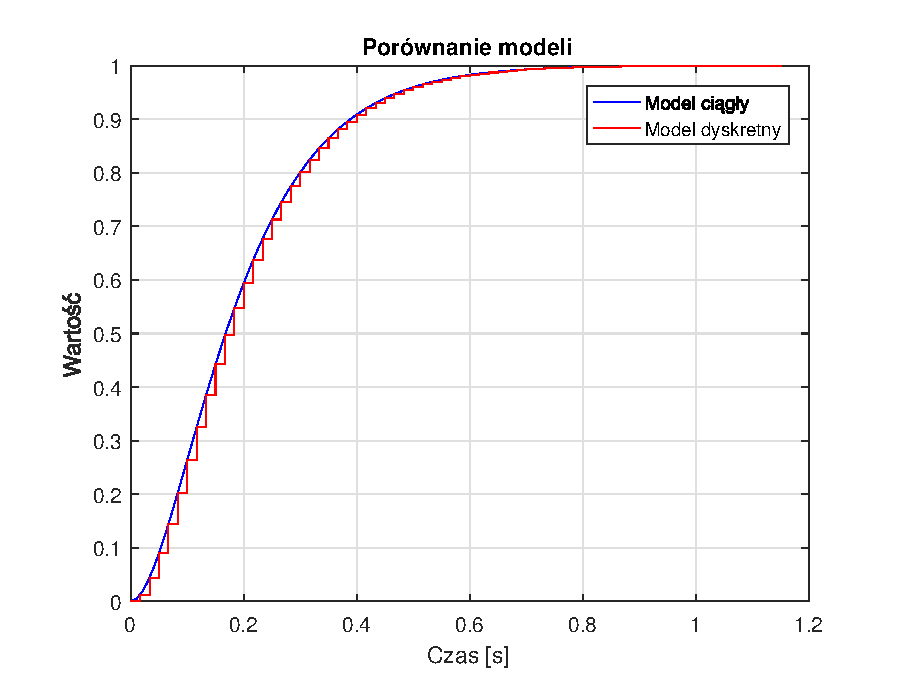
\includegraphics[width=4in]{comp.eps}
	\caption{Porównanie modelu ciągłego oraz odpowiadającego mu dyskretnego.}
	\label{fig:comp}
\end{figure}
%TODO referencja -zrobione.

Na podstawie powyższego wykresu można wnioskować, że wyliczony model jest poprawny.
Należy jednak zwrócić uwagę na fakt, że w rzeczywistym układzie występują dodatkowo opóźnienia, które nie zostały uwzględnione w modelu.
Na to opóźnienie składa się np. czas przesłania ramki obrazu z kamery do karty ewaluacyjnej lub komunikacja między elementami systemu.
%TODO jakie ? -zrobione.
Z tego względu model nie będzie idealnie odpowiadał działaniu rzeczywistego układu.

\paragraph*{}
Kompletny model układu postanowiono zaimplementować w programie \textit{Simulink}. Przedstawiony został na rysunku \ref{fig:simulink}. Zostało w nim uwzględnione:
\begin{itemize}
\item Nasycenie wartości zadanej serwomechanizmów
\item Przeliczanie współrzędnych śledzonego obiektu na kąty
\item Obliczanie szerokości impulsów wysyłanych do serwomechanizmu
\item Kwantyzację liczby pikseli i szerokości impulsów
\end{itemize}

\begin{figure}[h]
	\centering
	\includegraphics[width=4in]{Simulink.jpg}
	\caption{Model układu zrealizowany w programie \textit{Simulink}.}
	\label{fig:simulink}
\end{figure}
%TODO referencja ? -zrobione.

\section{Projekt regulatora}
\label{sec:projektregulatora}

W układzie nie ma czujnika pozycji serwomechanizmów, więc algorytm regulacji musi bazować na wyjściu z poprzedniej iteracji.
Algorytmem, który działa w ten sposób jest prędkościowy (przyrostowy) regulator PID.
Zaimplementowany regulator ma następującą postać:
\begin{equation}
u(k)-u(k-1)=P \cdot (e(k)-e(k-1))+I \cdot e(k)+D \cdot (e(k)-2e(k-1)+e(k-2))
\end{equation}
Został on zrealizowany w programie \textit{Simulink}, co przedstawiono na rysunku \ref{fig:przyrostowy}.

\begin{figure}[h]
	\centering
	\includegraphics[width=4in]{Przyrostowy.jpg}
	\caption{Realizacja przyrostowego regulatora PID.}
	\label{fig:przyrostowy}
\end{figure}
%TODO ref. -zrobione.

Na podstawie odpowiedzi modelu dobrano następujące wartości parametrów:
\begin{equation}
P=0.4
\end{equation}
\begin{equation}
I=0.1
\end{equation}
\begin{equation}
D=0.05
\end{equation}

\begin{figure}[H]
	\centering
	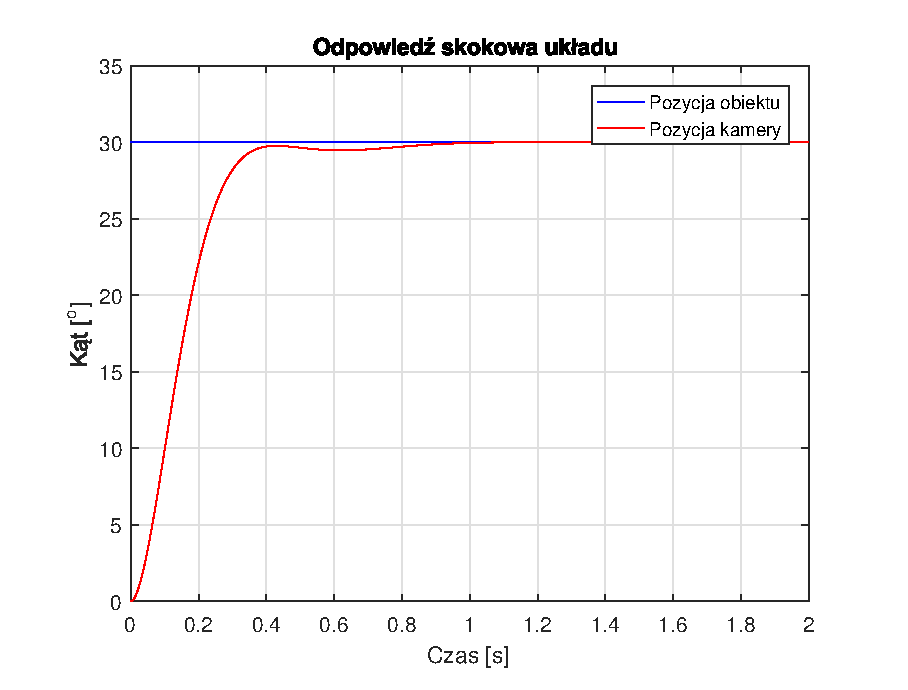
\includegraphics[width=3.4in]{sim_step.eps}
	\caption{Odpowiedź skokowa układu z dobranym regulatorem.}
\label{fig:sim_step}
\end{figure}
%TODO ref. -zrobione.

\begin{figure}[H]
	\centering
	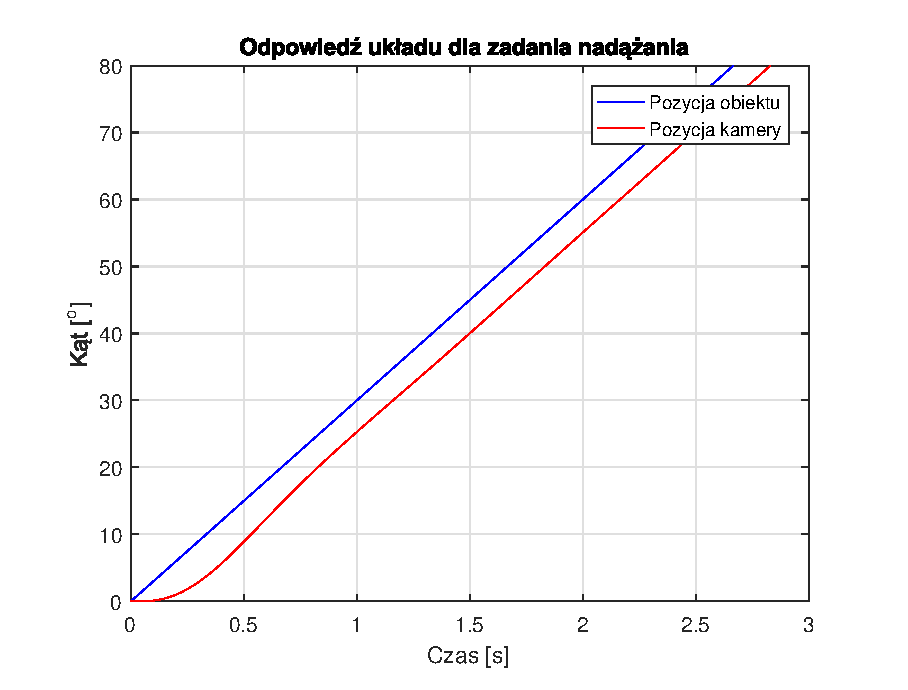
\includegraphics[width=3.4in]{sim_ramp.eps}
	\caption{Odpowiedź układu dla zadania nadążania.}
\label{fig:sim_ramp}
\end{figure}

Na rysunku \ref{fig:sim_step} pokazano odpowiedź skokową układu.
Widoczna jest szybka reakcja na skokową zmianę pozycji śledzonego obiektu.
Na rysunku \ref{fig:sim_ramp} pokazano odpowiedź układu dla zadania nadążania.
Zauważyć można, że w tym wypadku obecny jest uchyb ustalony.
Aby się go pozbyć konieczne byłoby zastosowanie w układzie regulatora wyższego rzędu, otrzymanego poprzez dodanie podwójnego członu całkującego do poprzednio rozważanego regulatora.
%TODO coś gram nie OK. -zrobione.
Mogłoby to zwiększyć przeregulowanie i wprowadzić większe oscylacje.
W efekcie pogorszona zostałaby odpowiedź skokowa układu.
Dlatego postanowiono pozostać przy zaproponowanym wcześniej rozwiązaniu.
Użyte parametry mogą zostać skorygowane w rzeczywistym układzie w zależności od rezultatów i wpływu pominiętych efektów.
%TODO niejasne, ale to dlaczego nie zastosować tego całkowania ? -zrobione.
%MK: Dodałem krótkie wyjaśnienie dlaczego z tego zrezygnowałem. Zaproponowane rozwiązanie przetestowałem w simulinku i udało mi się usunąć uchyb dla zadania nadążania, ale nie potrafiłem dobrać takich nastaw, żeby usunąć około 4-stopniowe przeregulowanie i oscylacje, które się pojawiły. Pomyślę nad rozwiązaniem tego w przyszłości pewnie, ale teraz nie chciałem na to tracić czasu. Inną sprawą jest brak metod doboru nastaw dla takiego regulatora. PID przyrostowy jest dość popularny i opisany, więc można spróbować zastosować jakąś metodę doboru nastaw (próbowałem z PID Tune w Simulinku, ale to nie działało dobrze).